\documentclass[a4wide]{report}

\usepackage{amsmath}
\usepackage[a4paper, total={7in, 10.2in}]{geometry}
\usepackage{graphicx}
\usepackage[portuguese]{babel}
\usepackage[utf8]{inputenc}


\begin{document}

\noindent
{\bf Rafael V. Cacilhas  - Relatório 12 e 13 (\today)}

\vspace{0.5cm}

\section*{Exercício 1}

\subsection*{a) }
Como a interação é local a diferença de energia depende apenas da interação do sítio $\nu$ com seus vizinhos mais próximos:


\begin{equation*}
\Delta E = E_{novo} - E{velho} 
\end{equation*} 

\begin{equation*}
J\left( s^{\nu}_{m,n}.s^{\nu}_{m+1,n} + s^{\nu}_{m,n}.s^{\nu}_{m-1,n}  +s^{\nu}_{m,n}.s^{\nu}_{m,n+1}  +s^{\nu}_{m,n}.s^{\nu}_{m,n-1}\right) - J\left( s^{\nu'}_{m,n}.s^{\nu}_{m+1,n} + s^{\nu'}_{m,n}.s^{\nu}_{m-1,n}  +s^{\nu'}_{m,n}.s^{\nu}_{m,n+1}  +s^{\nu'}_{m,n}.s^{\nu}_{m,n-1} \right)
\end{equation*} 
Como $s^{\nu'} = -s^{\nu}$, temos:
\begin{equation*}
\Delta E  =2J s^{\nu}_{m,n}.\left( s^{\nu}_{m+1,n} + s^{\nu}_{m-1,n}  +s^{\nu}_{m,n+1} + s^{\nu}_{m,n-1}\right)
\end{equation*} 

\subsection*{b) }
Feito nos programas alfa1.f90 até alfa5.f90 localizados na pasta 1. 

\subsection*{c) }
Os resultados estão na Figura \ref{1c}. Existe uma grande diferença no valor de $\tau$ para a energia e magnetização para $\alpha = 2$, o que talvez pode ser explicado devido ao fato de que em $\alpha = 2 $ o sistema transitou entre os dois estados ferromagnéticos, ou seja, $M = 1$ e $M = -1$, o que não aconteceu para os outros $\alpha$. Este fato está explícito nos histogramas na próxima alternativa.

\begin{figure}[!htb]
\centering
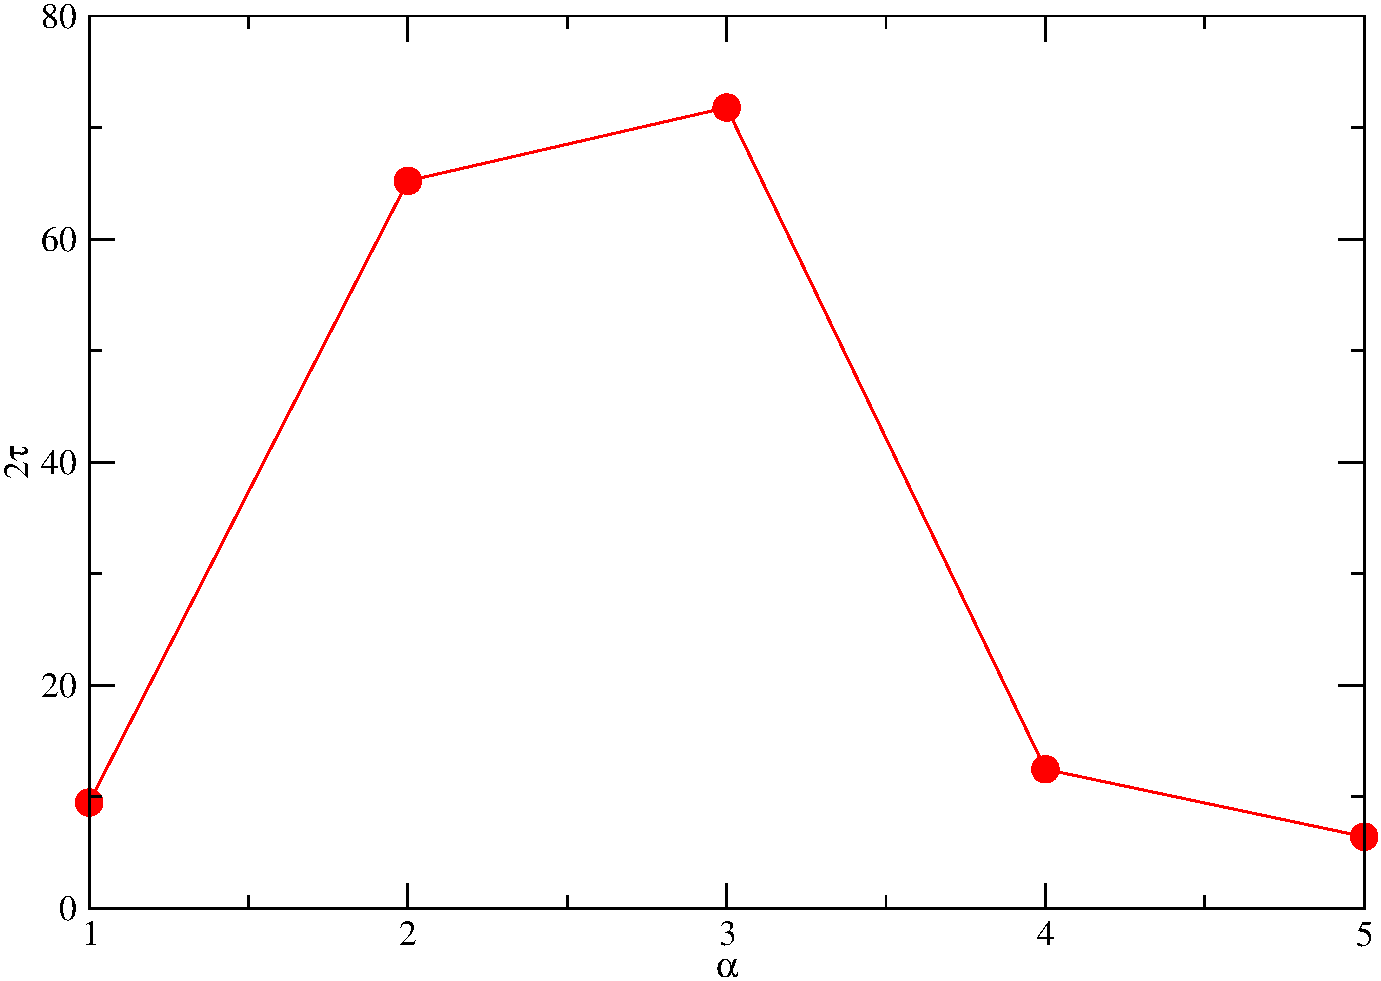
\includegraphics[width=0.32\textwidth]{2tau.pdf}
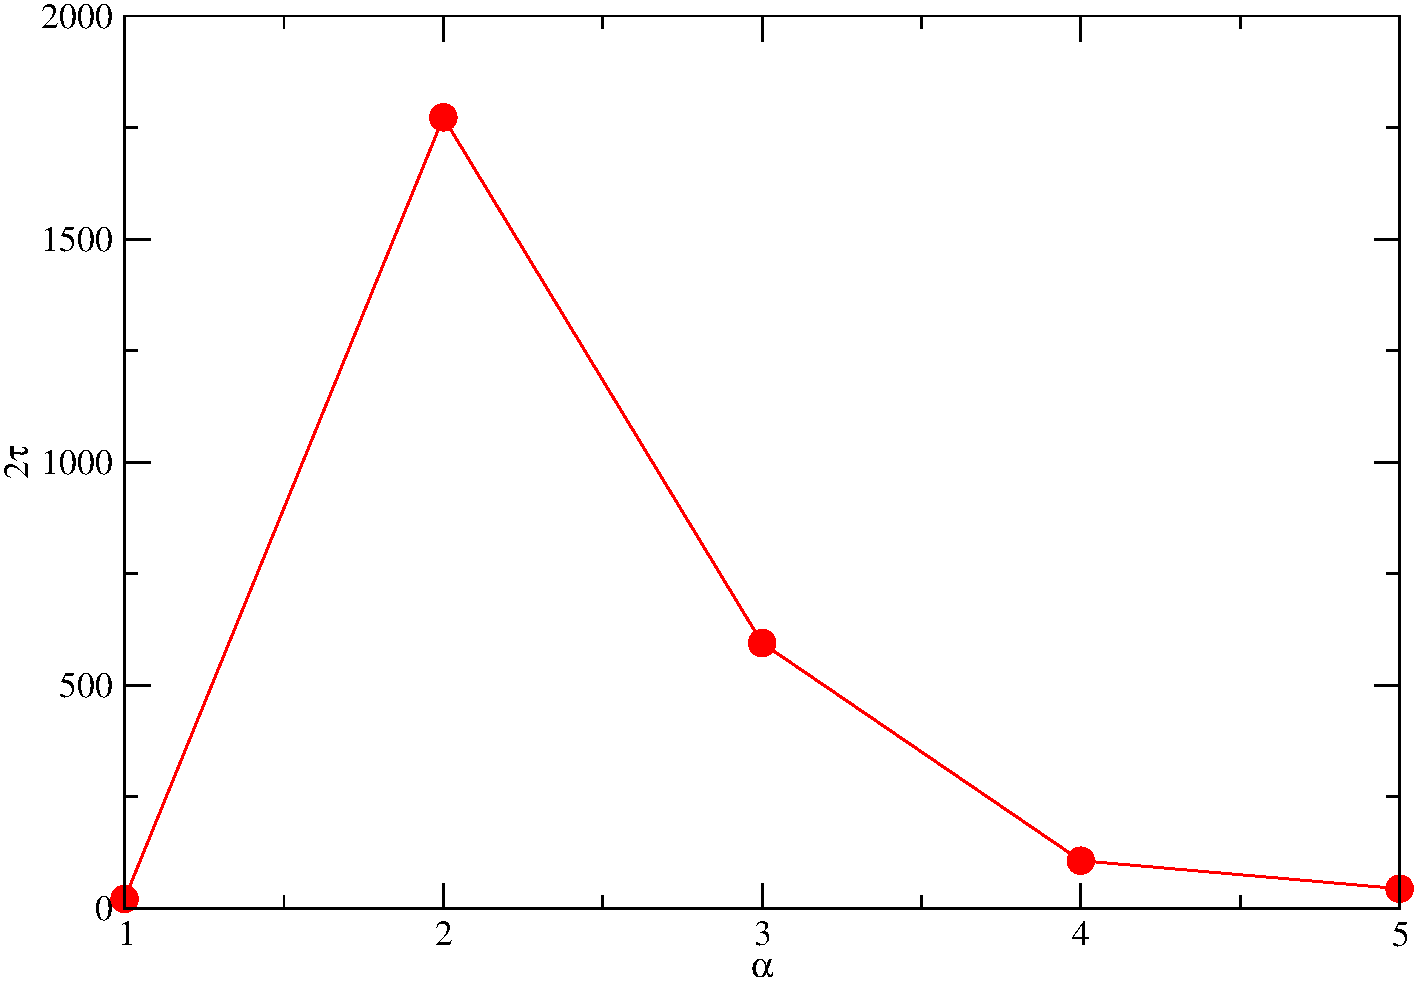
\includegraphics[width=0.32\textwidth]{2tau_mag.pdf}
\caption{2$\tau$ em função de $\alpha$ para a energia (esquerda) e magnetização (direita).  }
\label{1c}
\end{figure}

\subsection*{d) }
Os histogramas para energia e magnetização podem ser vistos na Figura \ref{1d}. Note que para $\alpha = 2$ o sistema possui magnetização perto dos dois extremos, o que mostra que os dois estados ferromagnéticos foram visitados muitas vezes. 
\begin{figure}[!htb]
\centering
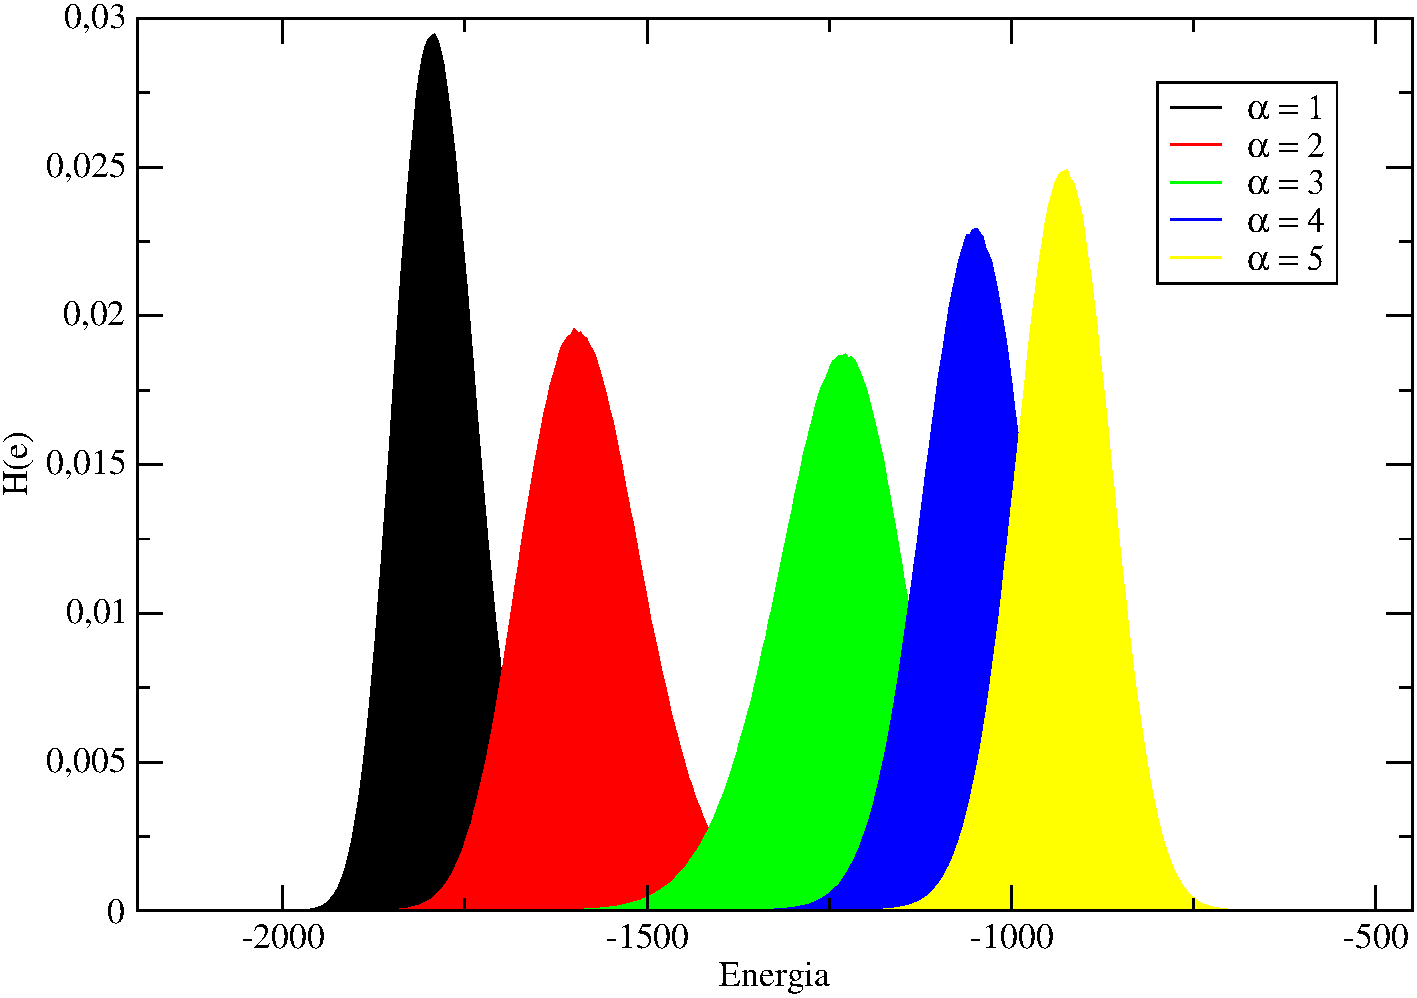
\includegraphics[width=0.32\textwidth]{energia.pdf}
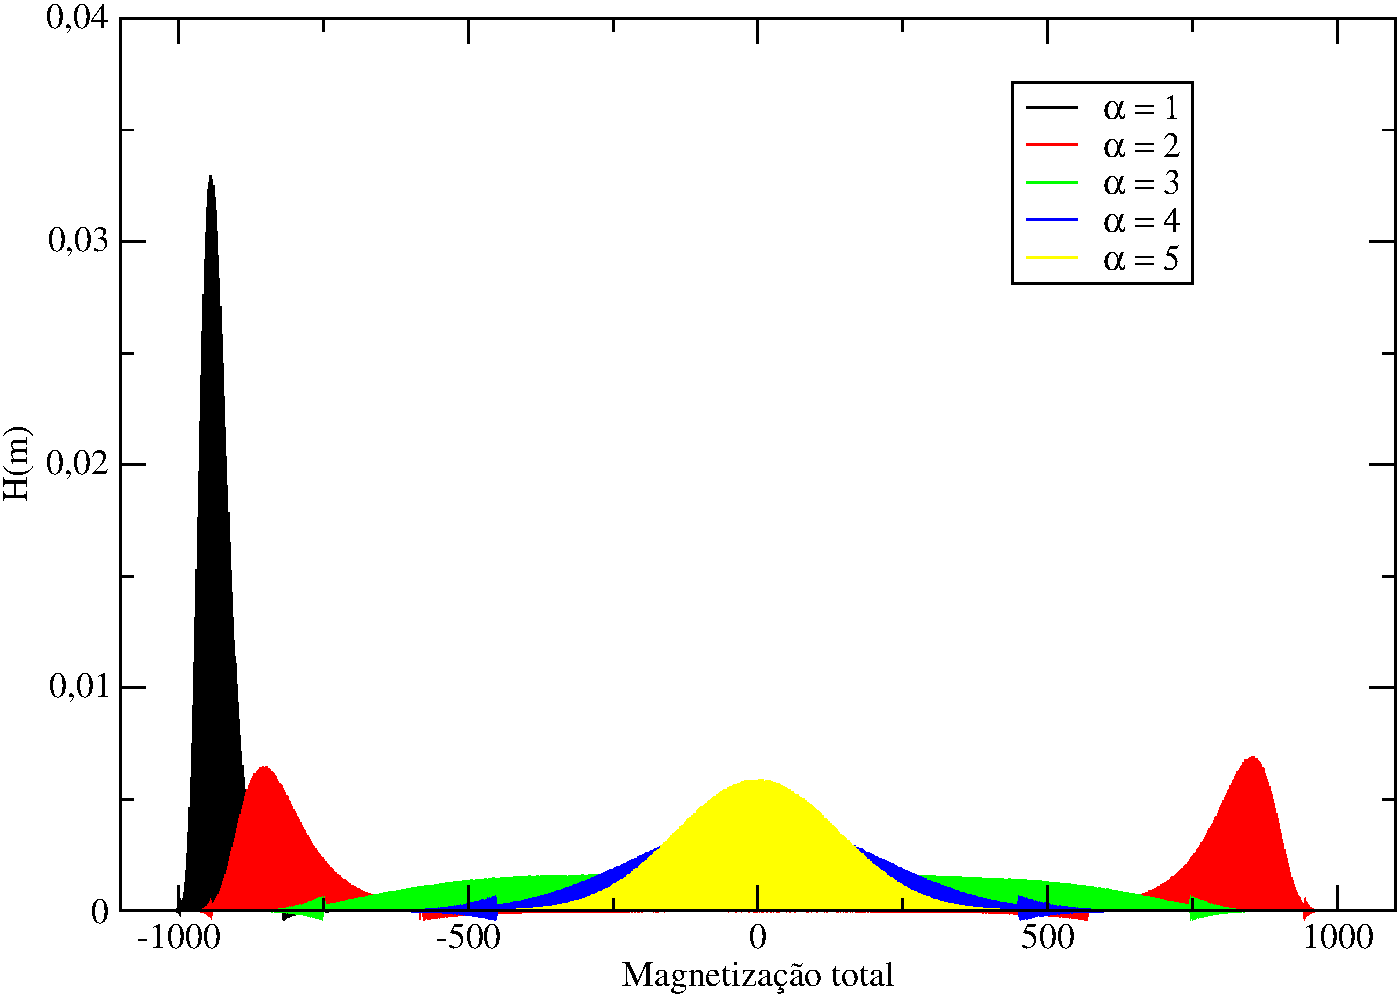
\includegraphics[width=0.32\textwidth]{mag.pdf}
\caption{Distribuição de energia e de magnetização em função dos passos de Monte Carlo.}
\label{1d}
\end{figure}

\subsection*{e)}
O programa começou a ser feito na pasta Análise/e.f90 , mas os resultados não foram adequados e foram omitidos.

\subsection*{h) }
Na Figura  \ref{1h} estão plotadas configurações típicas para cada $\alpha$.
\begin{figure}[!htb]
\centering
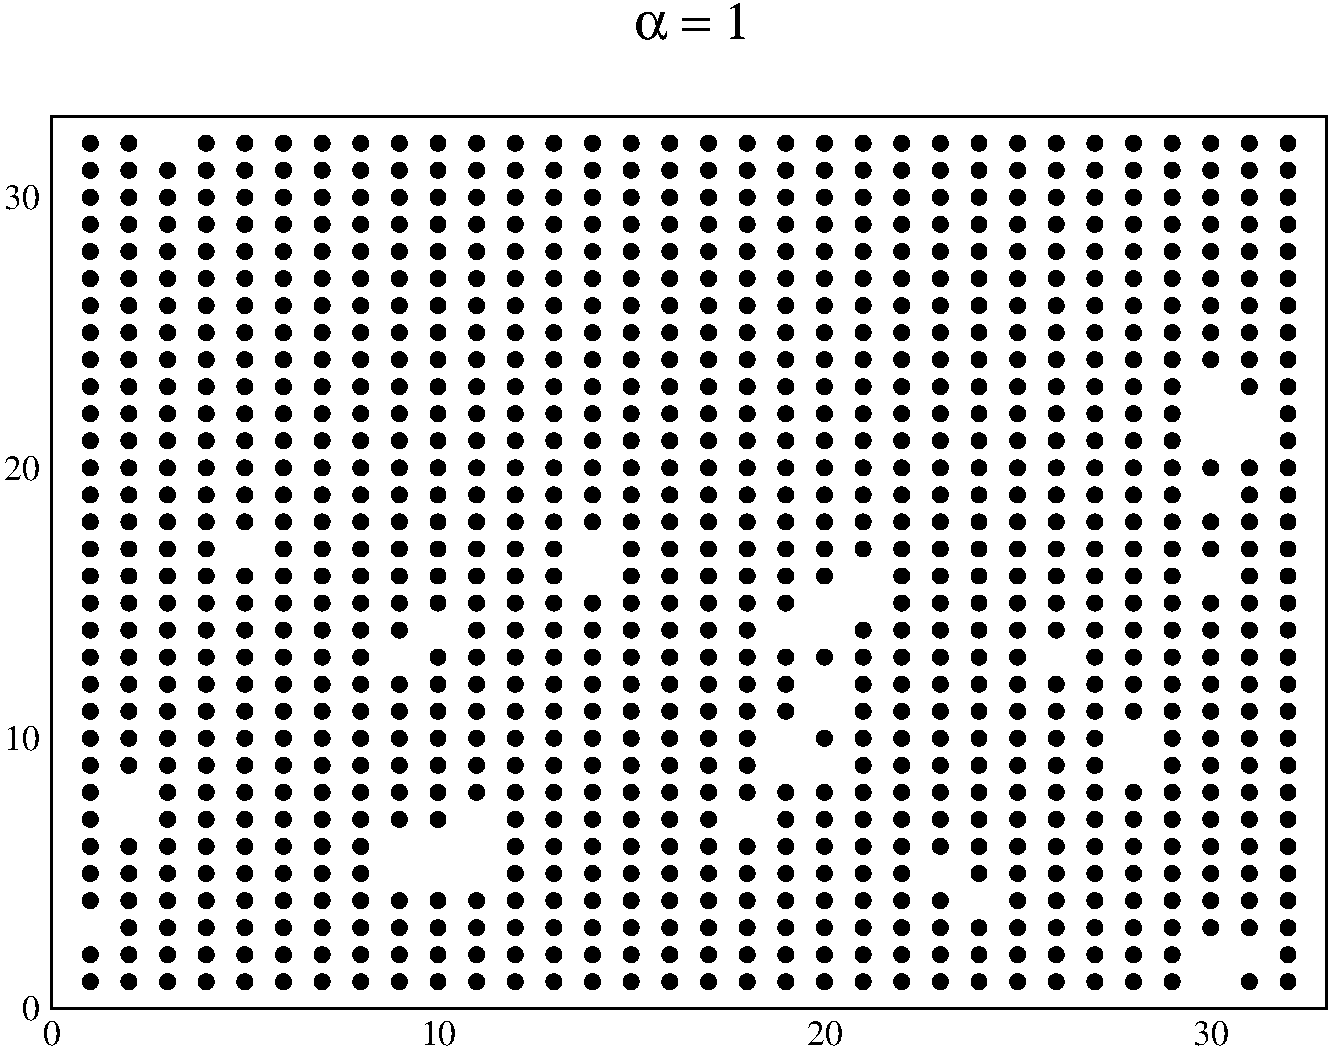
\includegraphics[width=0.32\textwidth]{1.pdf}
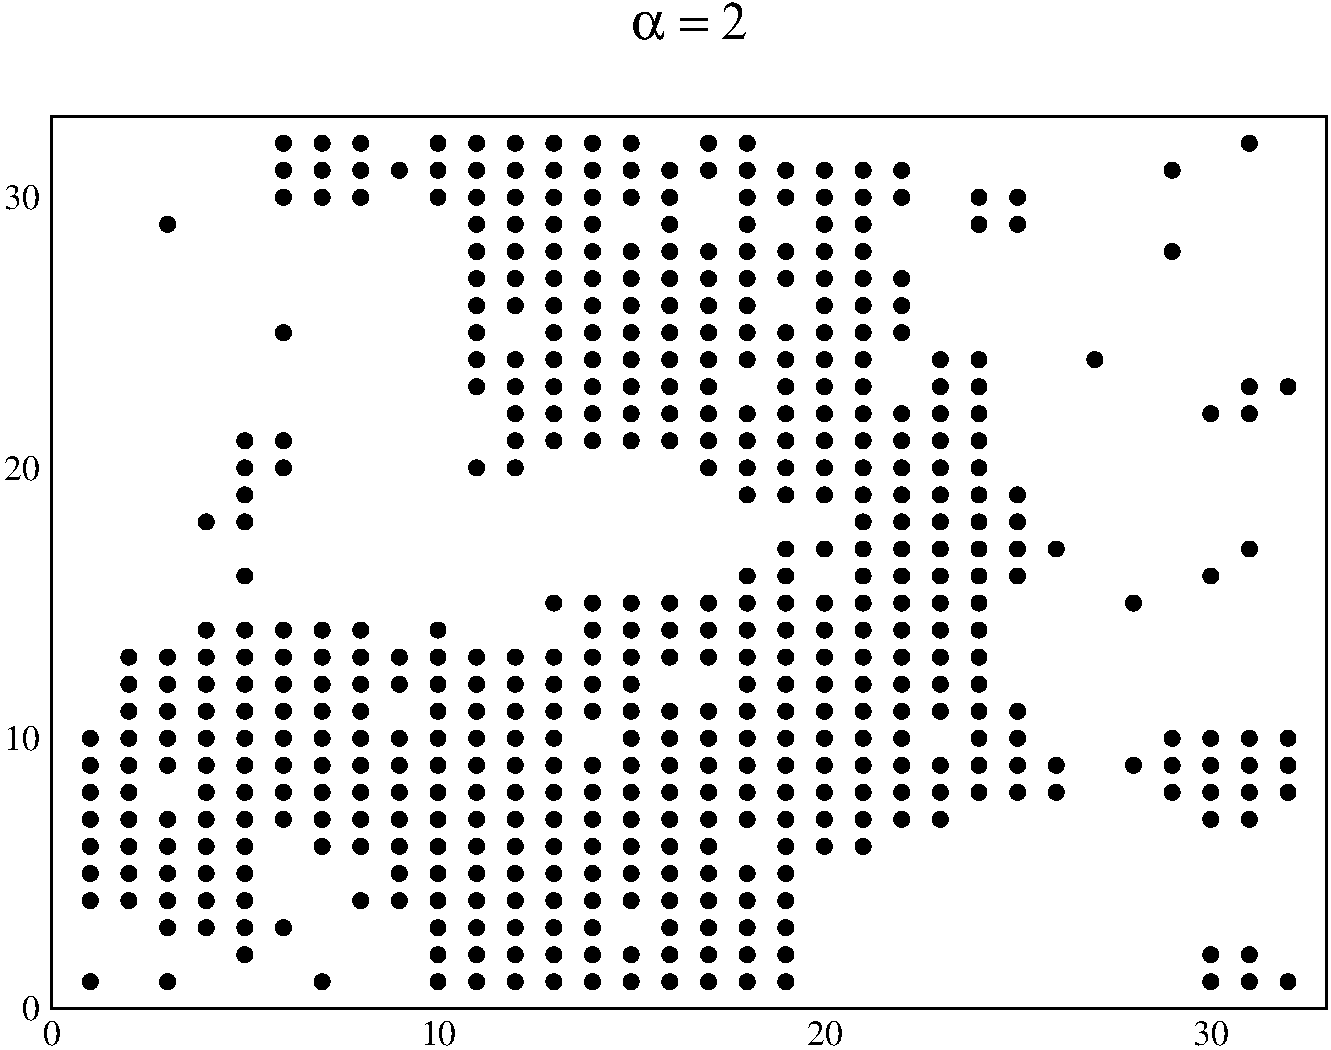
\includegraphics[width=0.32\textwidth]{2.pdf}
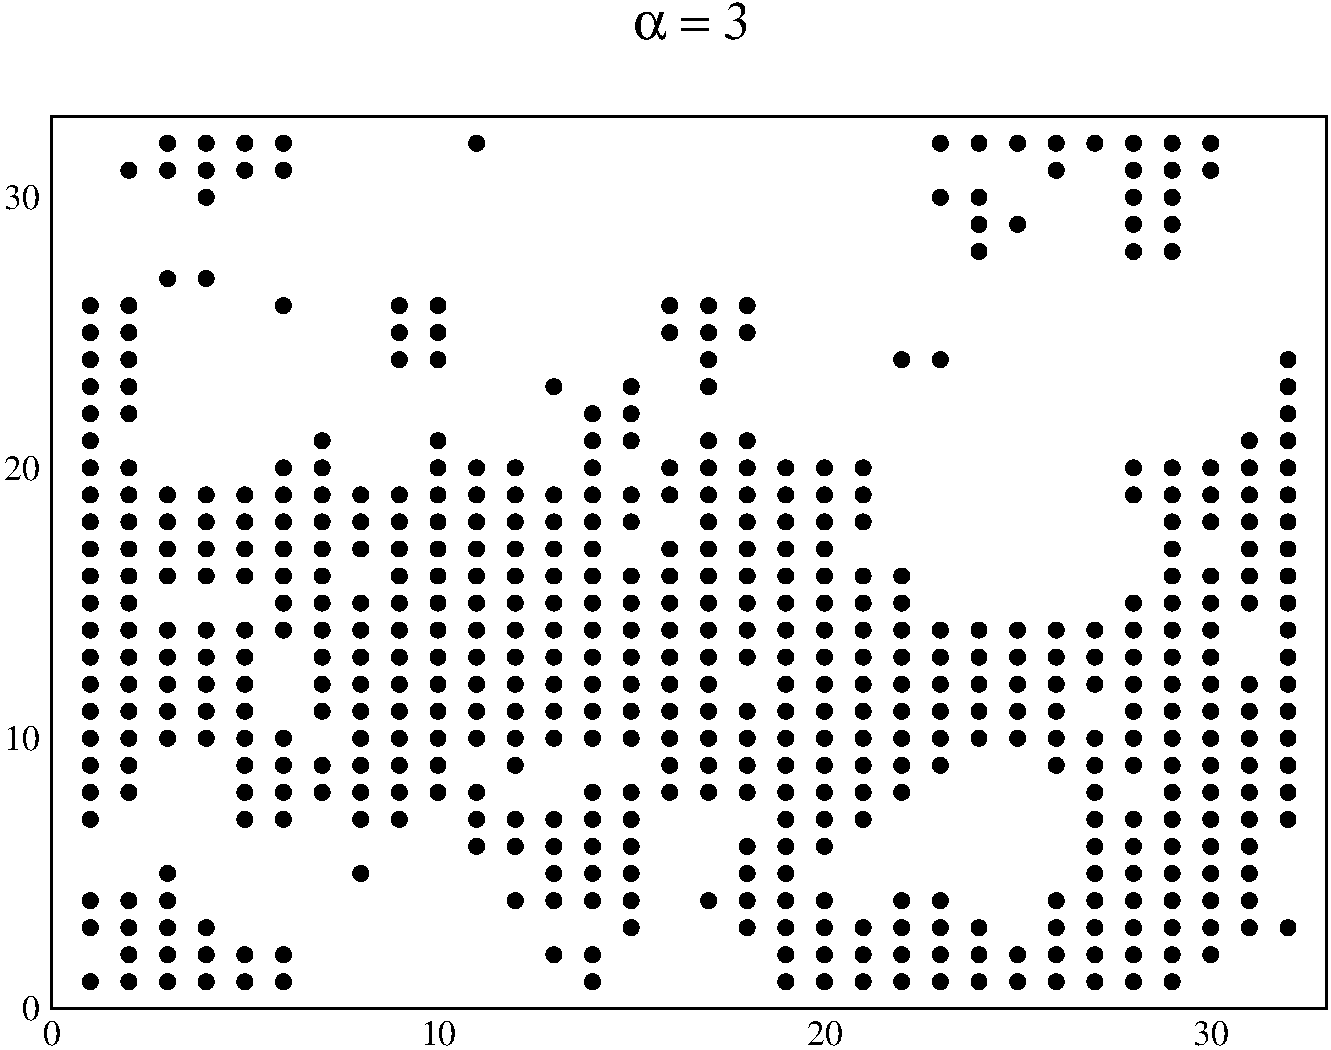
\includegraphics[width=0.32\textwidth]{3.pdf}
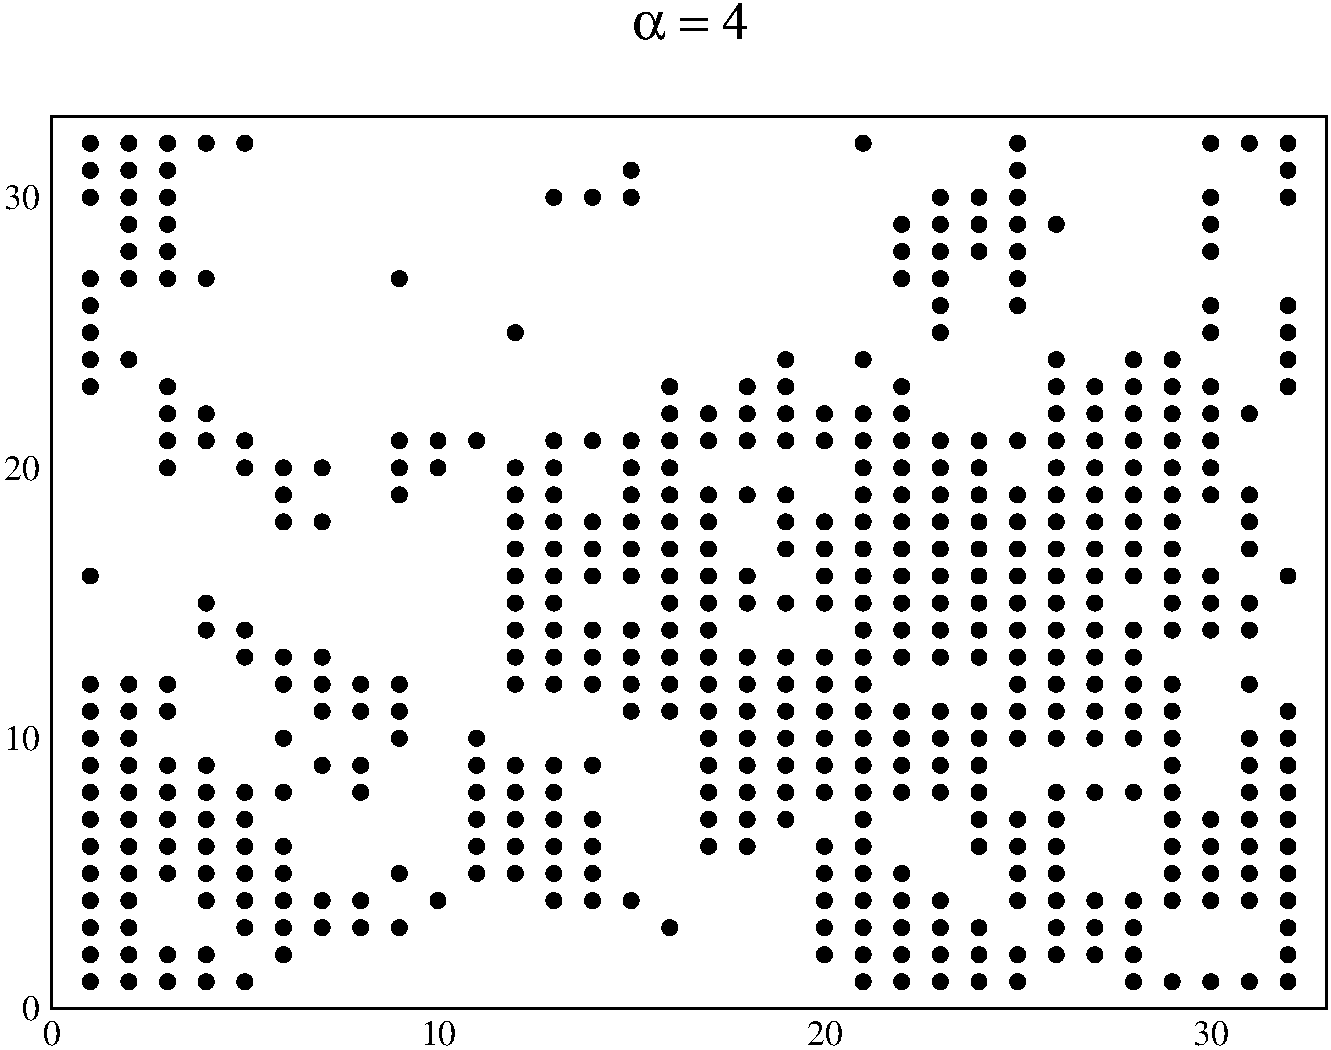
\includegraphics[width=0.32\textwidth]{4.pdf}
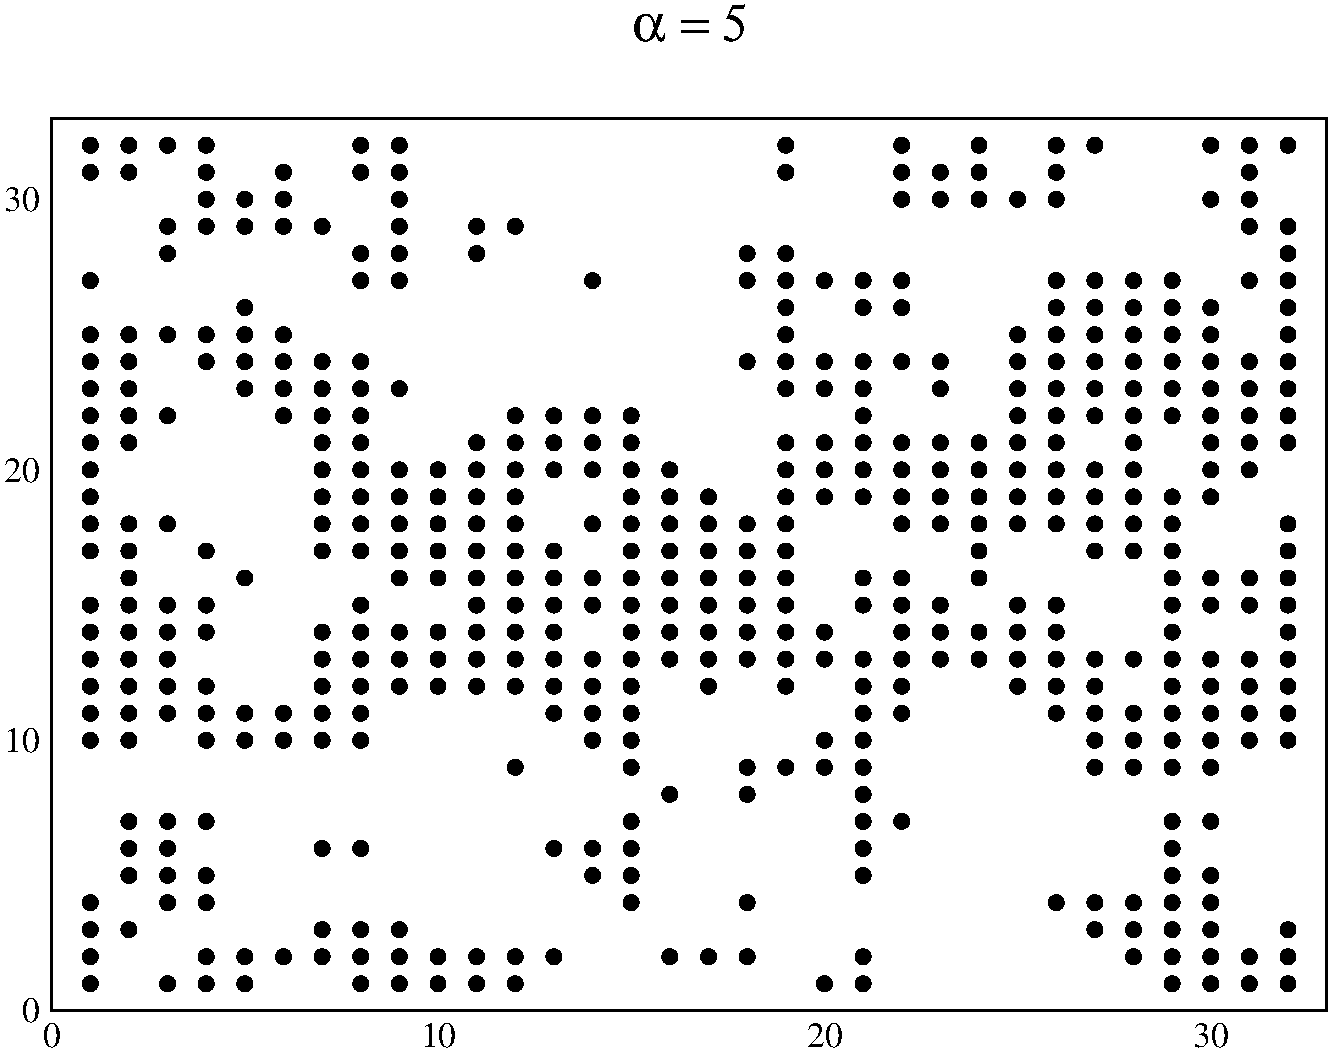
\includegraphics[width=0.32\textwidth]{5.pdf}
\caption{Configurações relevantes para cada temperatura $\alpha$.}
\label{1h}
\end{figure}

\section*{Exercício 2}
\subsection*{a)}
Feito no programa 2.f90 em sua respectiva pasta.
\subsection*{b)}
Para a energia obtivemos um valor de  2$\tau_{energia} = 1.04$ e para a magnetização foi obtido um valor de 2$\tau_{mag} = 1.31$.

\subsection*{c)}
Na Figura \ref{2c} temos os histogramas de energia e magnetização. O fato de não ser uma distribuição constante mostra que o programa não foi feito corretamente.
\begin{figure}[!htb]
\centering
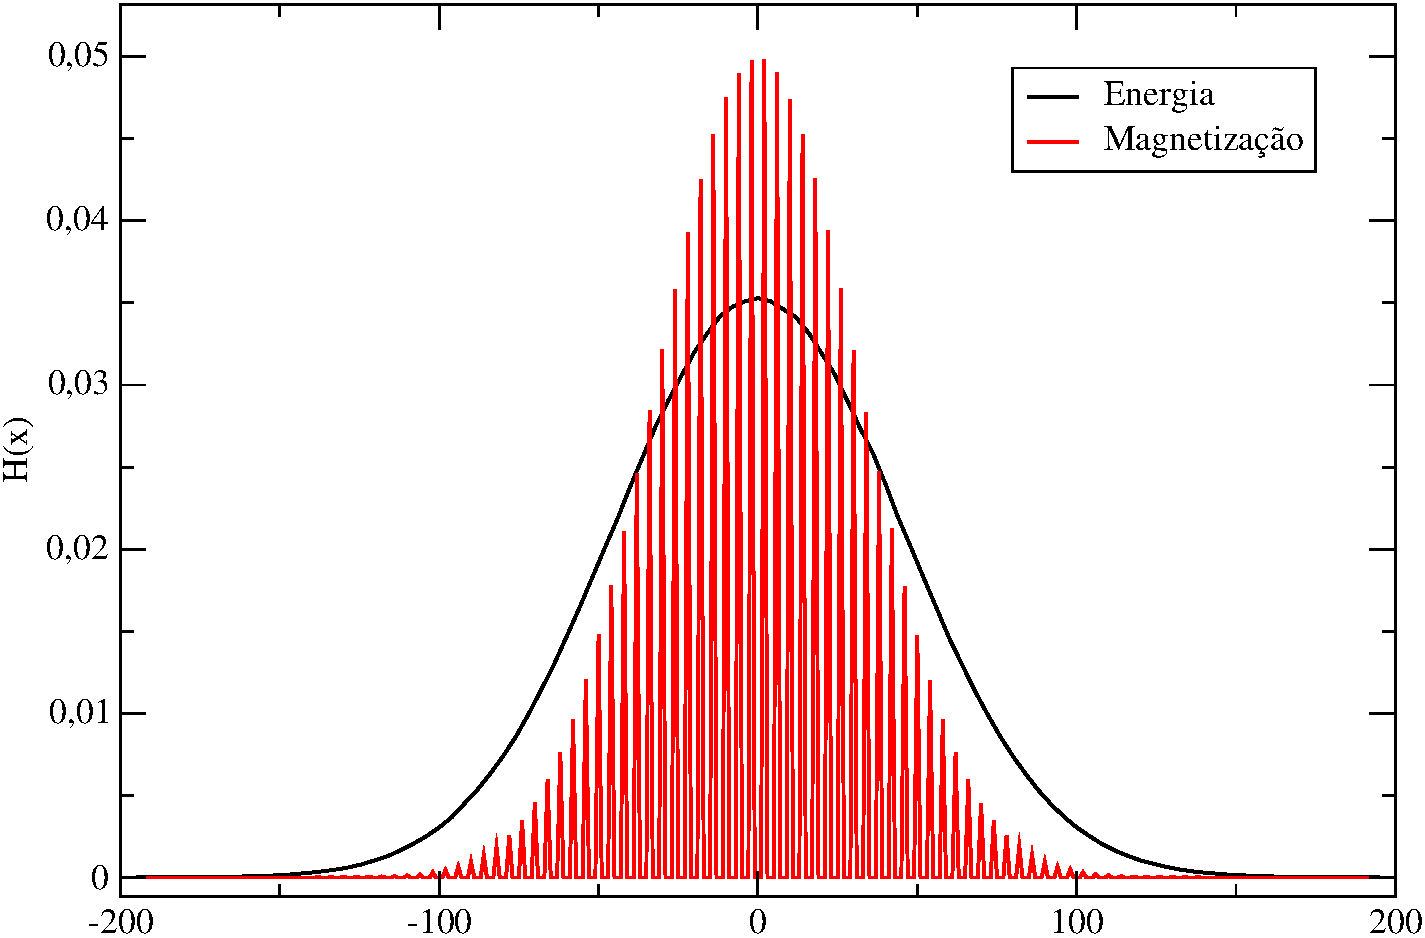
\includegraphics[width=0.32\textwidth]{mag2.pdf}
\caption{Histograma da energia e da magnetização.}
\label{2c}
\end{figure}


\end{document}